\section{Requirements}\label{sec:requirements}
In order to do model-based testing with GGs, stimuli and responses have to be obtained from the GG. ATM uses an IOSTS, where the instantiated switch relations represent a stimulus to or a response from the SUT. The rule transitions in an IOGTS are similar to the transitions in an IOLTS. First, the GG must be extended to an IOGG by indicating for each transformation rule whether it is of the input or output type. Then the IOGG can be explored to an IOGTS. The input/output rule transitions of the IOGTS can be used as the abstract stimuli and responses.

One requirement for the design is the possibility to measure coverage statistics. The exploration of a GG can be done in two ways: \textit{on the fly}, rule transitions are explored only when chosen by ATM, or \textit{offline}, the GG is first completely explored and then sent to ATM. On-the-fly model exploration works well on large and even infinite models. However, coverage statistics cannot be calculated with this technique. The number of states (graphs) and rule transitions the model has when completely explored are not known, so a percentage cannot be derived. As coverage statistics are an important metric, the offline model exploration is chosen for GRATiS.

Another requirement is efficiency. An IOGTS can potentially be infinitely large, due to the range of data values. A model that is more efficient with data values is an STS. The setup of GRATiS is therefore to transform the IOGG directly to an IOSTS. Note that the first requirement is met, because locaton and switch relation coverage can be calculated on the IOSTS.

\section{General setup}\label{sec:general-setup}
GRATiS uses GROOVE as a replacement of the IOSTS in ATM. Figure~\ref{fig:tooling} shows this graphically. GROOVE has several exploration strategies for exploring a GG to a GTS. GRATiS introduces two new strategies, the \textit{remote exploration strategy} and the \textit{symbolic exploration strategy}. The 'Exploration Strategy' is an exploration strategy in GROOVE such as the Breadth-First exploration strategy. The remote, symbolic and GROOVE exploration strategy form a chain where the possible rule transitions are passed down and the chosen rule transition is passed back up. The symbolic strategy transforms the GG to an STS based on the explored rule transitions. The remote exploration strategy waits until the IOSTS is done and then sends it to ATM. 'a' is the start of a new collaboration chain, representing the normal flow of ATM as depicted in Figure~\ref{fig:axini_tool}.

\begin{figure}[ht]
  \begin{center}
    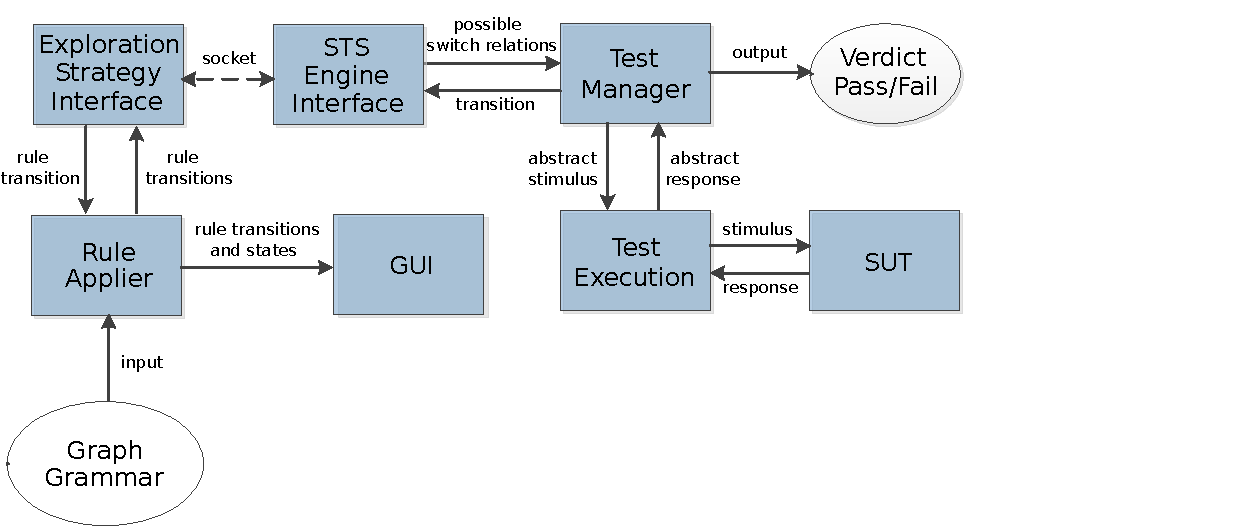
\includegraphics[width=\textwidth]{tooling.pdf}
  \end{center}
  \caption{The GRATiS design: replacing the STS with GROOVE}
  \label{fig:tooling}
\end{figure}
